\setcounter{secnumdepth}{-1}

\chapter{Background}
\section{Windows Security Landscape} 
Microsoft Windows is the most widely used desktop operating system in the world, making it a prime target for cyberattacks. 
To protect users, Windows offers a \textbf{layered security architecture}, including:

\begin{table}[H]
    \centering
    \begin{tabular}{|p{5cm}|p{10cm}|}
        \hline
        \textbf{Layer} & \textbf{Description} \\
        \hline
        Windows Defender Antivirus & Signature-based scanning, real-time file monitoring, heuristic behavior analysis \\
        \hline
        Windows Defender Firewall & Network filtering and application traffic rules \\
        \hline
        Windows Defender Exploit Guard & Memory protections, attack surface reduction, folder access control \\
        \hline
        Windows Event Logging & Logs process creation, network events, and privilege escalation \\
        \hline
        AMSI (Antimalware Scan Interface) & Allows inspection of PowerShell scripts, macros, and dynamic code at runtime \\
        \hline
        EDR (Endpoint Detection and Response) & Advanced behavioral analysis, telemetry collection, and threat correlation (often third-party tools) \\
        \hline
    \end{tabular}
    \caption{Windows Security Layers and Their Functions}
    \label{tab:windows_security_layers}
\end{table}

However, attackers have evolved equally \textbf{advanced evasion techniques} to \textbf{bypass or confuse these security layers}. This project focuses on evaluating how well these defenses stand up to modern \textbf{stealth techniques} in real-world tests.

\begin{figure}[H]
    \centering
    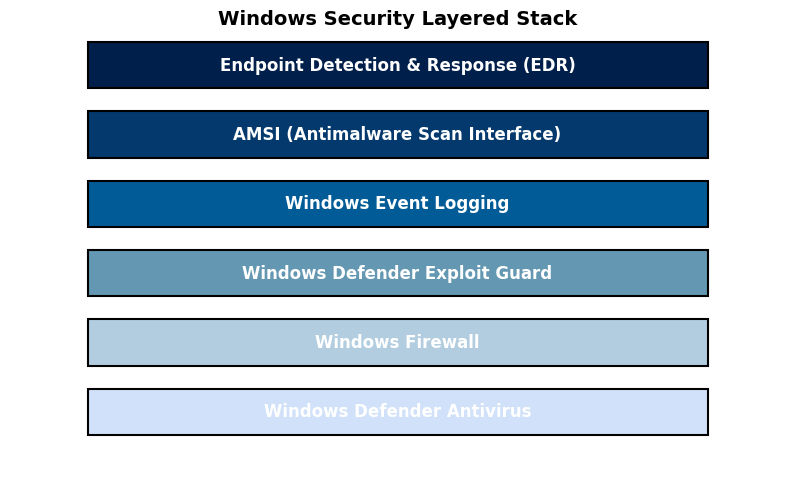
\includegraphics[width=\textwidth]{Pictures/windowssecuritylayer.png}
    \caption{Diagram showing the layered security stack in Windows (Defender, Firewall, AMSI, EDR)}
    \label{fig:windowssecuritylayer}
\end{figure}

This diagram illustrates the layered architecture of Windows security, starting from basic real-time antivirus scanning up to advanced behavioral analysis provided by EDR solutions. These layers work together to detect known threats, suspicious behaviors, and emerging attacks by combining file scanning, process monitoring, memory inspection, and telemetry analysis.

\section{Evasion Techniques in Windows}

Modern attackers rarely use obvious malware files. Instead, they hide within \textbf{legitimate processes} or exploit \textbf{trusted system tools}. This project focuses on:

\subsection{1. Hidden Command Execution with LOLBins}

\textbf{Living Off the Land Binaries (LOLBins)} are legitimate Windows binaries misused for malicious purposes. Since they are signed by Microsoft, they \textbf{bypass many security checks}.

\begin{table}[H]
    \centering
    \begin{tabular}{|l|l|}
        \hline
        \textbf{LOLBin} & \textbf{Abuse Example} \\
        \hline
        rundll32.exe & Executes DLL functions directly (payload injection) \\
        mshta.exe & Runs malicious HTML/JS payloads \\
        certutil.exe & Downloads payloads over HTTPS \\
        regsvr32.exe & Loads malicious COM objects remotely \\
        \hline
    \end{tabular}
    \caption{Common LOLBins and their abuse techniques}
\end{table}

Example command:
\begin{verbatim}
rundll32.exe shell32.dll,Control_RunDLL payload.dll
\end{verbatim}

\subsection{2. Keyloggers — Silent Data Capture}

A \textbf{keylogger} hooks into \textbf{low-level keyboard events} to capture every keystroke. Simple keyloggers use:
\begin{verbatim}
SetWindowsHookEx(WH_KEYBOARD_LL, KeyboardProc, NULL, 0);
\end{verbatim}

More advanced ones \textbf{inject into trusted processes} like `explorer.exe`, making them \textbf{blend into normal system behavior}. Detection focuses on:

\begin{itemize}
    \item Monitoring unexpected process hooks.
    \item Detecting exfiltration of logged keystrokes.
    \item Correlating process behavior and file writes.
\end{itemize}

\subsection{3. Process Injection \& Hollowing}

This is one of the most powerful evasion techniques. The attacker injects malicious code into a \textbf{trusted process} like \texttt{svchost.exe}, effectively hiding the malware.

\begin{table}[H]
    \centering
    \begin{tabular}{|l|l|}
        \hline
        \textbf{Injection Type} & \textbf{Explanation} \\
        \hline
        DLL Injection & Loads malicious DLL into another process \\
        Process Hollowing & Starts process in suspended state, hollows it, injects malicious code \\
        Thread Hijacking & Injects code into existing process threads \\
        \hline
    \end{tabular}
    \caption{Types of Process Injection Techniques}
\end{table}

% Example API sequence:
% \begin{verbatim}
% CreateProcess() -> SuspendThread() -> VirtualAllocEx() -> 
% WriteProcessMemory() -> ResumeThread()
% \end{verbatim}


\usetikzlibrary{shapes.geometric, arrows}

\tikzstyle{startstop} = [rectangle, rounded corners, minimum width=3cm, minimum height=1cm, text centered, draw=black, fill=yellow!30]
\tikzstyle{process} = [rectangle, minimum width=3cm, minimum height=1cm, text centered, draw=black, fill=green!15]
\tikzstyle{decision} = [diamond, minimum width=3cm, minimum height=1cm, text centered, draw=black, fill=orange!30]
\tikzstyle{arrow} = [thick,->,>=stealth]

\begin{center}
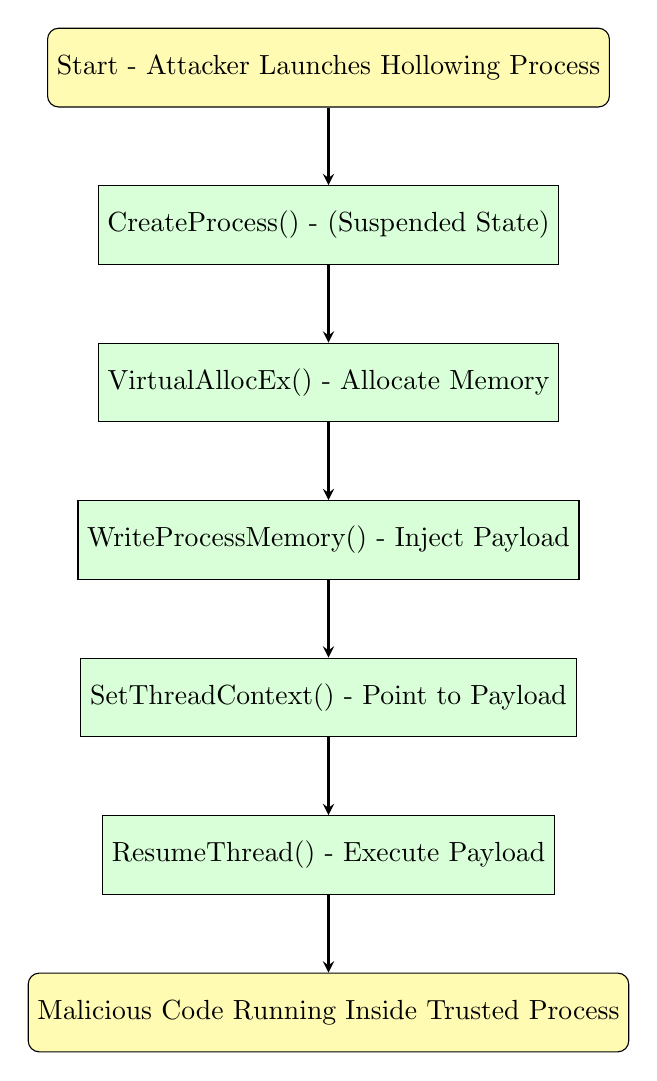
\begin{tikzpicture}[node distance=2cm]

% Nodes
\node (start) [startstop] {Start - Attacker Launches Hollowing Process};
\node (createproc) [process, below of=start] {CreateProcess() - (Suspended State)};
\node (allocmem) [process, below of=createproc] {VirtualAllocEx() - Allocate Memory};
\node (writemem) [process, below of=allocmem] {WriteProcessMemory() - Inject Payload};
\node (changectx) [process, below of=writemem] {SetThreadContext() - Point to Payload};
\node (resumethread) [process, below of=changectx] {ResumeThread() - Execute Payload};
\node (end) [startstop, below of=resumethread] {Malicious Code Running Inside Trusted Process};

% Arrows
\draw [arrow] (start) -- (createproc);
\draw [arrow] (createproc) -- (allocmem);
\draw [arrow] (allocmem) -- (writemem);
\draw [arrow] (writemem) -- (changectx);
\draw [arrow] (changectx) -- (resumethread);
\draw [arrow] (resumethread) -- (end);

\end{tikzpicture}
\end{center}

\begin{center}
    \textbf{Process Hollowing Flowchart} \\
\end{center}  

This flowchart illustrates the sequence of steps involved in a process hollowing attack. 
The attacker first launches a process in a suspended state using \texttt{CreateProcess()}. 
Next, memory in the target process is allocated using \texttt{VirtualAllocEx()}, and the malicious payload is written into this memory using \texttt{WriteProcessMemory()}. 
The attack then modifies the thread context using \texttt{SetThreadContext()} to redirect execution to the malicious payload. 
Finally, the suspended thread is resumed using \texttt{ResumeThread()}, allowing the payload to execute within the context of the trusted process.
This technique allows malware to blend into legitimate processes, making detection by traditional security tools more difficult.


\subsection{4. Backdoor Creation \& Persistence Techniques}

Attackers want long-term access, so they use \textbf{persistence techniques} such as:

\begin{table}[H]
    \centering
    \begin{tabular}{|l|l|}
        \hline
        \textbf{Technique} & \textbf{Example} \\
        \hline
        Registry Run Key & Adds payload to HKCU\textbackslash Software\textbackslash Microsoft\textbackslash Windows\textbackslash CurrentVersion\textbackslash Run \\
        Scheduled Task & Creates hidden task running malware on boot \\
        Service Creation & Registers malware as a system service \\
        \hline
    \end{tabular}
    \caption{Persistence Techniques in Windows}
\end{table}


% \section*{Persistence Techniques and Real Examples}

% \begin{table}[H]
%     \centering
%     \begin{tabular}{|p{4cm}|p{7cm}|}
%         \hline
%         \textbf{Technique} & \textbf{Real Command Example} \\
%         \hline
%         Registry Run Key & 
%         \lstinline|reg add "HKCU\Software\Microsoft\Windows\CurrentVersion\Run" /v MyApp /t REG_SZ /d "C:\malware\payload.exe"| \\
%         \hline
%         Scheduled Task & 
%         \lstinline|schtasks /create /tn "Updater" /tr "C:\malware\payload.exe" /sc onlogon /ru SYSTEM| \\
%         \hline
%         Service Creation & 
%         \lstinline|sc create MaliciousService binPath= "C:\malware\payload.exe"| \\
%         \hline
%         Startup Folder Drop & 
%         Copy payload to: \lstinline|%APPDATA%\Microsoft\Windows\Start Menu\Programs\Startup\| \\
%         \hline
%     \end{tabular}
%     \caption{Common Persistence Techniques and Real Command Examples}
%     \label{tab:persistence_techniques}
% \end{table}


\begin{figure}[H]
    \centering
    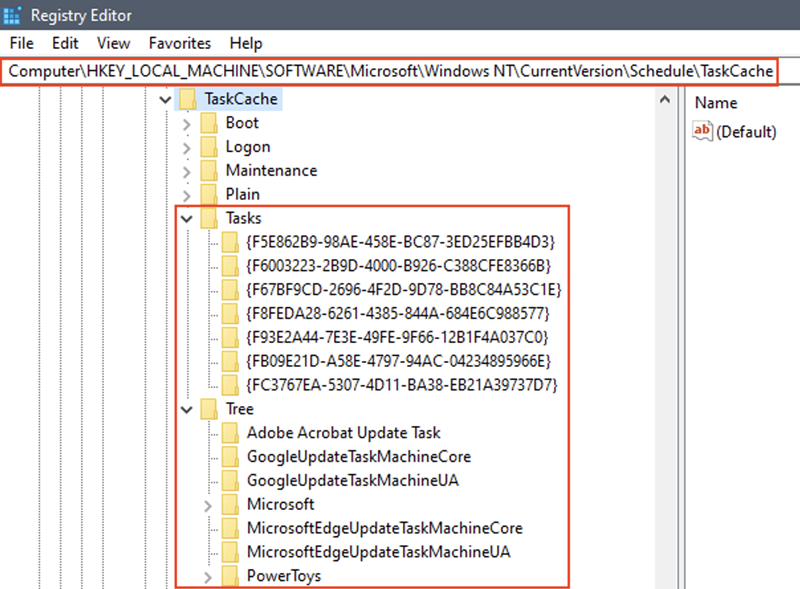
\includegraphics[width=0.8\textwidth]{Pictures/Fig1_Tarrask-malware-creates-new-registry-keys-along-with-the-creation-of-new-scheduled-tasks.png}
    \caption{Screenshot of malicious task created via \texttt{schtasks} command in Windows Task Scheduler}
    \label{fig:malicious_task_scheduler}
\end{figure}


Example command:
\begin{verbatim}
        schtasks /create /tn "Updater" /tr "C:\backdoor\payload.exe" /sc onlogon /ru SYSTEM
\end{verbatim}

\section{Defender and EDR — Strengths \& Weaknesses}

\subsection{1. Detection Methods Used}
\begin{itemize}
    \item Signature Matching: Known bad files, hashes
    \item Heuristic Analysis: Process behavior (e.g., spawning cmd.exe from Word)
    \item Log Analysis: Event logs (e.g., suspicious command lines)
    \item Memory Scanning: Scans process memory for injected code
    \item Network Monitoring: Detects unusual outbound connections
\end{itemize}

\subsection{2. Key Limitations}
\begin{table}[H]
    \centering
    \begin{tabular}{|l|l|}
        \hline
        \textbf{Limitation} & \textbf{Why it Matters} \\
        \hline
        Trusted Process Blind Spot & Signed Windows processes are trusted by default \\
        Fileless Attack Resistance & If malware never touches disk, signature scans miss it \\
        Log Overload & In noisy environments, alerts get buried \\
        Cross-Process Visibility & Process injection can bypass monitoring hooks \\
        \hline
    \end{tabular}
    \caption{Weaknesses in Defender and EDR}
\end{table}

\section{Why Real-World Testing Matters}

Lab tests often rely on known malware samples, but \textbf{real attackers hide in plain sight}:

\begin{itemize}
    \item PowerShell obfuscation
    \item Fileless payload delivery
    \item Encrypted Command \& Control (C2)
\end{itemize}

\begin{figure}[H]
    \centering
    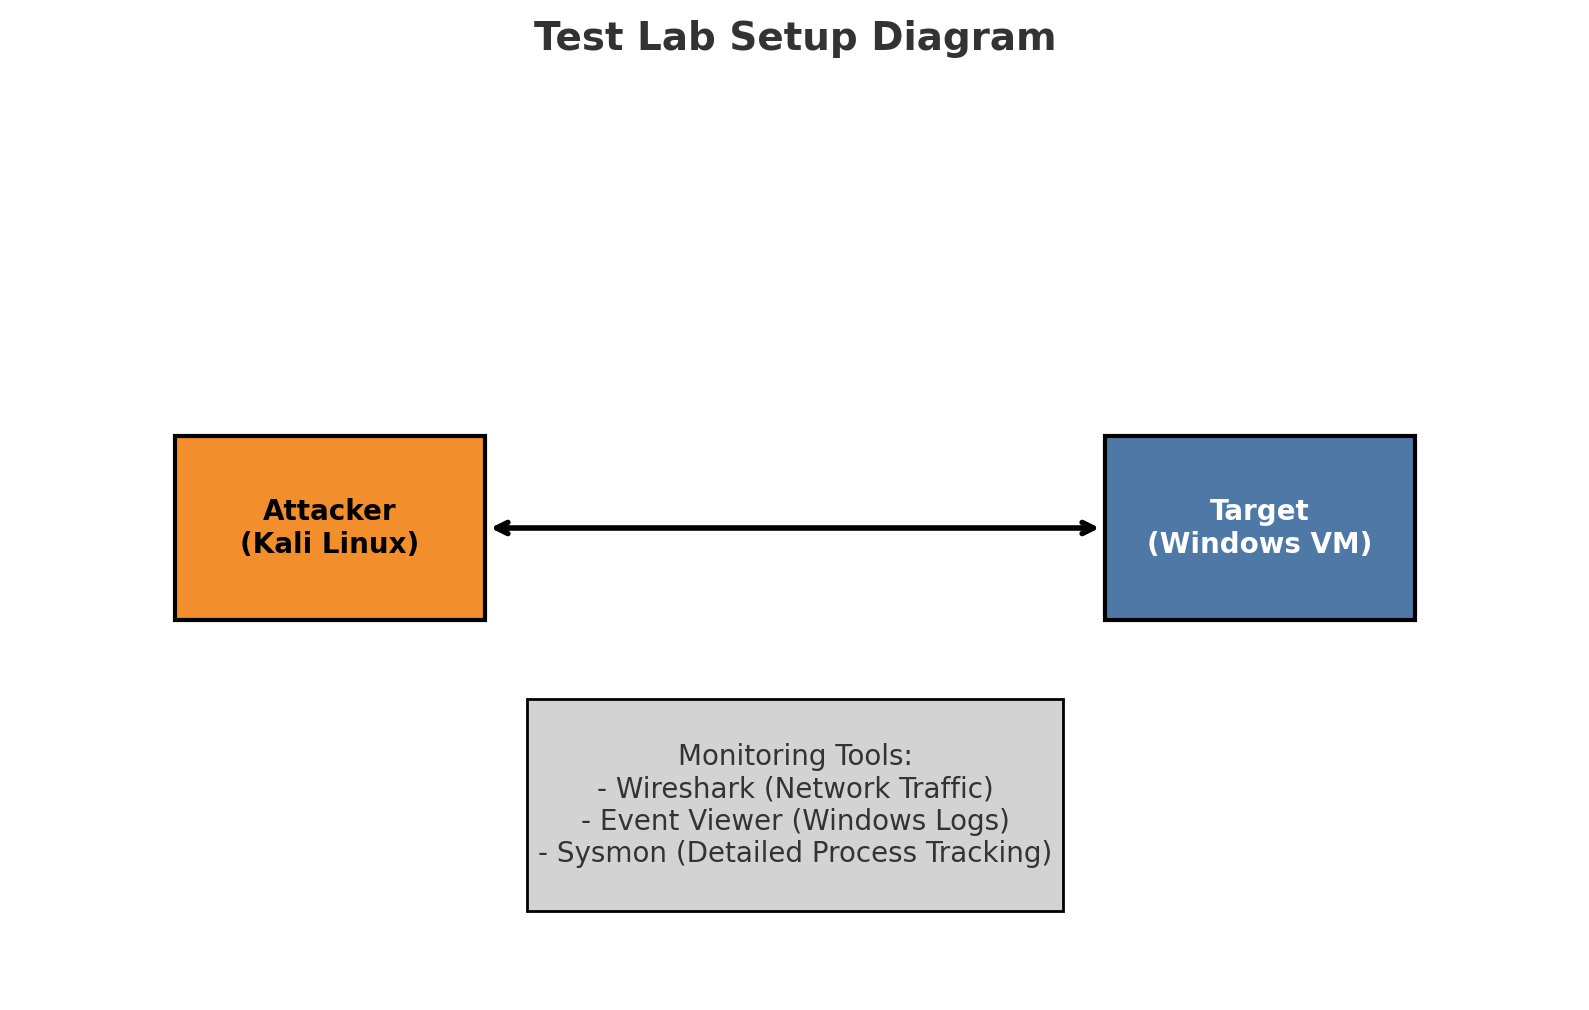
\includegraphics[width=0.8\textwidth]{Pictures/test_lab_env.png}
    \caption{Test Lab Setup: Attacker (Kali Linux) attacking Target (Windows) with monitoring via Wireshark, Event Viewer, and Sysmon}
    \label{fig:test_lab_setup}
\end{figure}

This project simulates these real-world \textbf{stealth techniques} to measure:

\begin{table}[H]
    \centering
    \begin{tabular}{|l|l|}
        \hline
        \textbf{Evaluation Metric} & \textbf{Explanation} \\
        \hline
        Detection Time & How fast is the initial detection? \\
        Detection Accuracy & How many techniques were detected? \\
        Alert Quality & Are alerts actionable, or just noise? \\
        \hline
    \end{tabular}
    \caption{Evaluation Metrics for Real-World Testing}
\end{table}
